\todoZ{3.1: Cover SO(3) parameterizations with quaternions, MRPs, and axis-angle representations}
\todoZ{3.1: Detail conversions, singularities, and representation choices for optimization versus sampling}
\todoX{3.1: Define the Modified (Craig) Denavit-Hartenberg convention for the 7-DOF manipulator}
\todoX{3.2: Formulate spacecraft attitude dynamics on SO(3)}
\todoX{3.2: Formulate 7-DOF robotic manipulator dynamics}
\todoX{3.2: Define state, input, and kinodynamic constraint envelopes for both systems}
\todoX{3.2: Specify actuator, joint, angular-velocity, and angular-acceleration limits}
\todoX{3.3: Formalize the continuous-time optimal control problem}
\todoX{3.3: Transcribe the OCP into a discrete nonlinear program}
\todoX{3.3: Detail B-spline parameterization of state and control trajectories}
\todoX{3.3: Describe the IPOPT interface, discretization, and constraint handling}
\todoX{3.4: Present MC-GBO, RRT*-GBO, P-HO, and IPSO consistently}
\todoX{3.4: Describe naive versus uniform SO(3) sampling}
\todoX{3.4: Define Arm7 sampling bounds}
\todoX{3.5: Detect kinodynamic and boundary violations along B-spline trajectories}
\todoX{3.5: Locally densify time-grid nodes to enforce feasibility}
\todoX{3.6: Prove and analytically verify the unconstrained SO(3) maneuver baseline}

\section{Methodology}
\label{sec:methodology}

This chapter is to be completed according to the following checklist.

\subsection{Mathematical Foundations \& Representations}
\label{sec:methodology-foundations}
\begin{itemize}
	\item[$\square$] \textbf{Manipulator kinematics:} Define the Modified (Craig) Denavit--Hartenberg (DH) parameter convention used for the 7-DOF manipulator.
\end{itemize}

\subsubsection{Attitude Representations}
\label{sec:attitude-representations}
The attitude of a rigid body in \ac{3-D} space can be represented using a myriad of parameterizations, each with its own advantages and limitations. 
Common representations include rotation matrices, quaternions, \ac{MRPs}, Euler angles, and axis--angle representations.
Rotation matrices are a classic choice for representing attitudes offering a singularity-free, intuitive geometric interpretation, with a linear mapping of vectors. 
However, they are over-parameterized with nine elements versus the minimal three required to describe rotations. 
This increases the computational load. 
Quaternions offer a more compact, four-element singularity-free representation of rotations compared to rotation matrices, but suffer from double cover and an unintuitive physical meaning of the parameters.
\ac{MRPs} are a three-element representation--making them a minimal and efficient description of rotations--that avoid the double-cover issue of quaternions but contain singularities at 360 degrees.
Euler angles are also a minimal representation with very intuitive geometric interpretation, but they suffer from gimbal lock.
Finally, axis--angle representations describe rotations using a rotation axis and an angle about that axis. 
They provide a clear geometric interpretation and are minimal, but they become singular at zero rotation whereby the axis-of-rotation becomes ill-defined.

\paragraph{Coordinate Systems}
\label{par:coordinate-systems}
To describe the attitude of a rigid body, it is first essential to describe the coordinate systems involved. Throughout this description, we consider two coordinate systems:
\begin{itemize}
	\item[$\bullet$] \textbf{Inertial frame:} A reference frame fixed in space, notated by the subscript $\mathbf{i}$. 
                                                The inertial frame serves as the global reference frame upon which all other reference frames, positions, and orientations are defined in relation to.
	\item[$\bullet$] \textbf{Body frame:} A coordinate system fixed to the rigid body, denoted by the subscript $\mathbf{b}$, used to describe the orientation of the body relative to itself.
\end{itemize}

Vectors are expressed with respect to a specific coordinate system, with the preceding superscript indicating the frame the vector is expressed in, e.g., ${}^{\mathbf{i}}\mathbf{x}$ denotes a vector $\mathbf{x}$ expressed in the inertial frame.

While in principle, the inertial frame is fixed in space, in practice a convenient approximation is to consider merely a very slowly moving frame, such as one attached to the Earth or center of the Solar system.

\paragraph{Rotation Matrices}
\label{par:rotation-matrices}
A rotation matrix--also known as a \ac{DCM} \cite{Schuster93}--is a matrix which, when multiplied with a vector expressed in one coordinate frame, transforms it into another coordinate frame. 
Alternatively, it can be seen as an operator that rotates a vector while preserving its length \cite{Diebel06}.
The former description describes a \emph{passive} rotation, where the coordinate frame is rotated relative to a fixed vector, while the latter describes an \emph{active} rotation, where the vector itself is rotated within a fixed coordinate frame.
The passive rotation conventions will be adopted throughout this work.
A second important convention is also important to clarify: This work defines these matrices as mapping the body frame to the inertial frame--as opposed to the other way around.
An example of the relative orientation of the inertial and body frames is shown in \cref{fig:dcm-2d}.

\begin{figure}[htbp]
	\centering
	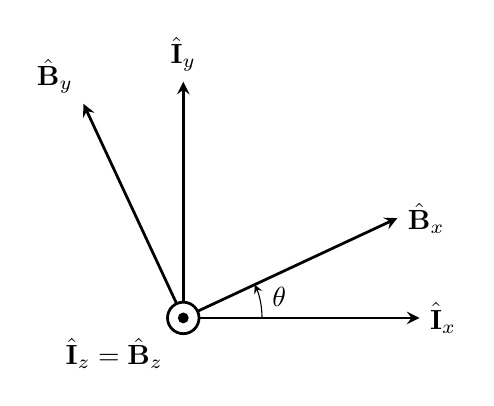
\begin{tikzpicture}[>=stealth, line width=1pt, scale=2.5]
    \def\thetaAngle{25}
    \def\axisLen{1.2}

    % Inertial frame
    \draw[->] (0,0) -- (\axisLen,0) node[right] {$\hat{\mathbf{I}}_x$};
    \draw[->] (0,0) -- (0,\axisLen) node[above] {$\hat{\mathbf{I}}_y$};

    % Body frame rotated by theta Angle
    \draw[->] (0,0) -- (\thetaAngle:\axisLen) node[right] {$\hat{\mathbf{B}}_x$};
    \draw[->] (0,0) -- (90+\thetaAngle:\axisLen) node[above left] {$\hat{\mathbf{B}}_y$};

    % Common z-axis, pointing out of the page
    \filldraw[fill=white, draw=black] (0,0) circle (0.08);
    \filldraw[black] (0,0) circle (0.02);
    \node[anchor=north east] at (-0.05,-0.05) {$\hat{\mathbf{I}}_z = \hat{\mathbf{B}}_z$};

    % Rotation angle
    \draw[->, thin] (0.4,0) arc (0:\thetaAngle:0.4);
    \node at ({\thetaAngle/2}:0.5) {$\theta$};
\end{tikzpicture}

	\caption{Inertial frame $\{\hat{\mathbf{I}}_x, \hat{\mathbf{I}}_y, \hat{\mathbf{I}}_z\}$ and body frame $\{\hat{\mathbf{B}}_x, \hat{\mathbf{B}}_y, \hat{\mathbf{B}}_z\}$ rotated by angle $\theta$ about the common $z$-axis.}
	\label{fig:dcm-2d}
\end{figure}

Rotation matrices are the core mathematical representation used in this work to perform coordinate transformations of vectors, points, and coordinate frames. 
As such, a brief overview of their properties and usage is provided below.

The set of all proper orthogonal rotation matrices forms the \emph{special orthogonal group} \(\SO{3}\):

\begin{equation}
\SO{3} = \left\{ \mathbf{R} \in \mathbb{R}^{3 \times 3} \mid \mathbf{R}^\top \mathbf{R} = \mathbf{I}, \det(\mathbf{R}) = 1 \right\}.
\label{eq:so3-definition}
\end{equation}
\begin{equation}
\mathbf{R}^\top \mathbf{R} = \mathbf{I}
\quad \Longleftrightarrow \quad
\mathbf{R}^\top = \mathbf{R}^{-1}.
\label{eq:orthogonal-inverse}
\end{equation}

The elements of rotation matrices are referenced by their row and column indices:
\begin{equation}
\mathbf{R} = 
\begin{bmatrix}
r_{11} & r_{12} & r_{13} \\
r_{21} & r_{22} & r_{23} \\
r_{31} & r_{32} & r_{33}
\end{bmatrix}.
\label{eq:rotation-matrix-elements}
\end{equation}

Vector coordinate transformations are performed by premultiplying the \emph{vector} \(\mathbf{v} \in \Real^3\) by a rotation matrix:
\begin{equation}
    {}^{\text{i}}\mathbf{v} = \mathbf{R}_{\text{ib}} {}^{\text{b}}\mathbf{v}
\label{eq:vector-transformation}
\end{equation}
Here the vector \({}^{\text{b}}\mathbf{v}\) originally expressed in the body frame is transformed into the inertial frame \({}^{\text{i}}\mathbf{v}\) using the rotation matrix \(\mathbf{R}_{\text{ib}}\).
Equation \cref{eq:vector-transformation} highlights that rotation matrices provide a direct linear mapping of vectors via simple matrix multiplication.

Unlike vector transformations, transforming a \emph{point} \(\mathbf{x} \in \Real^3\) requires both rotation and translation, as points have a fixed position in space rather than just a direction and magnitude.
To demonstrate, consider a point \({}^{\text{b}}\mathbf{x}\) expressed in the body frame, the origin of the body frame being \({}^{\text{b}}\mathbf{x}_{\text{b}}\), and the origin of the inertial frame being \({}^{\text{i}}\mathbf{x}_{\text{i}}\). 
Its coordinates in the inertial frame \({}^{\text{i}}\mathbf{x}\) are obtained by applying both the rotation and translation:
\begin{equation}
    {}^{\text{i}}\mathbf{x} = \mathbf{R}_{\text{ib}} \left( {}^{\text{b}}\mathbf{x} - {}^{\text{b}}\mathbf{x}_{\text{b}} \right) + {}^{\text{i}}\mathbf{x}_{\text{i}} = \mathbf{R}_{\text{ib}} {}^{\text{b}}\mathbf{x} - {}^{\text{i}}\mathbf{x}_{\text{b}} + {}^{\text{i}}\mathbf{x}_{\text{i}} 
\label{eq:point-transformation}
\end{equation}
Naturally, the origins of the body and inertial frames expressed in their respective frames are zero vectors \(\mathbf{0}\) simplifying \cref{eq:point-transformation}:
\begin{equation}
    {}^{\text{i}}\mathbf{x} = \mathbf{R}_{\text{ib}} \left( {}^{\text{b}}\mathbf{x} - {}^{\text{b}}\mathbf{x}_{\text{b}} \right) = \mathbf{R}_{\text{ib}} {}^{\text{b}}\mathbf{x} - {}^{\text{i}}\mathbf{x}_{\text{b}} 
\label{eq:point-transformation-simplified}
\end{equation}

Multiple rotation matrices may be composed to represent successive rotations, multiplying from right to left.
If \(\mathbf{R}_{\text{ib}}\) maps vectors from the body frame to the inertial frame, and \(\mathbf{R}_{\text{bs}}\) maps vectors from the sensor frame to the body frame, then the composite rotation matrix \(\mathbf{R}_{\text{is}}\) mapping vectors from the sensor frame to the inertial frame is given by:
\begin{equation}
\mathbf{R}_{\text{is}} = \mathbf{R}_{\text{ib}} \mathbf{R}_{\text{bs}}
\end{equation}

Rotation matrices are also known as \ac{DCM}s because each element represents the cosine of the angle between the corresponding axes of the two coordinate frames.
\begin{equation}
    % write the dot product representaiton
    \mathbf{R}_{\text{ib}} = 
    \begin{bmatrix}
        \hat{\mathbf{I}}_x \cdot \hat{\mathbf{B}}_x & \hat{\mathbf{I}}_x \cdot \hat{\mathbf{B}}_y & \hat{\mathbf{I}}_x \cdot \hat{\mathbf{B}}_z \\
        \hat{\mathbf{I}}_y \cdot \hat{\mathbf{B}}_x & \hat{\mathbf{I}}_y \cdot \hat{\mathbf{B}}_y & \hat{\mathbf{I}}_y \cdot \hat{\mathbf{B}}_z \\
        \hat{\mathbf{I}}_z \cdot \hat{\mathbf{B}}_x & \hat{\mathbf{I}}_z \cdot \hat{\mathbf{B}}_y & \hat{\mathbf{I}}_z \cdot \hat{\mathbf{B}}_z
    \end{bmatrix}
\label{eq:DCM-dot-prod}
\end{equation}

Because the dot product of two unit vectors \(\hat{\mathbf{I}}\) and \(\hat{\mathbf{B}}\) is:
\begin{equation}
    \hat{\mathbf{I}}_i \cdot \hat{\mathbf{B}}_j = \|\hat{\mathbf{I}}_i\| \|\hat{\mathbf{B}}_j\| \cos\alpha_{ij} = \cos\alpha_{ij}, \quad i,j \in \{x,y,z\}
\label{eq:dot-product-definition}
\end{equation}

\cref{eq:DCM-dot-prod} may therefore be expressed in terms of the cosines of the angles between the corresponding axes.
Let \(\alpha_{ij}\) denote the angle between the inertial frame axis \(\hat{\mathbf{I}}_i\) and the body frame axis \(\hat{\mathbf{B}}_j\), 
corresponding respectively to row \(i\) and column \(j\) of the rotation matrix (where \(i,j \in \{x,y,z\} \)).
\begin{equation}
    \mathbf{R}_{\text{ib}} = 
    \begin{bmatrix}
        \cos\alpha_{xx} & \cos\alpha_{xy} & \cos\alpha_{xz} \\
        \cos\alpha_{yx} & \cos\alpha_{yy} & \cos\alpha_{yz} \\
        \cos\alpha_{zx} & \cos\alpha_{zy} & \cos\alpha_{zz}
    \end{bmatrix}
\label{eq:DCM-cos-alpha}
\end{equation}
\emph{example}: The equation of the rotation shown in \cref{fig:dcm-2d}
\begin{equation}
    \mathbf{R}_{\text{ib}} = 
    \begin{bmatrix}
        \cos\alpha & \cos(\pi/2+\alpha) & \cos(\pi/2) \\
        \cos(\pi/2-\alpha) & \cos\alpha & \cos(\pi/2) \\
        \cos(\pi/2) & \cos(\pi/2) & \cos(0)
    \end{bmatrix}
    =
    \begin{bmatrix}
        \cos\alpha & -\sin\alpha & 0 \\
        \sin\alpha & \cos\alpha & 0 \\
        0 & 0 & 1
    \end{bmatrix}
\end{equation}

We conclude with a brief discussion of the drawbacks and benefits of using rotation matrices for attitude representation.

\paragraph{Pros}
\begin{itemize}
    \item Direct Mapping: Rotation matrices provide a direct linear mapping of vectors via matrix multiplication.
    \item Singularity-Free: They are free from geometric singularities.
    \item Intuitive Kinematics: They provide a clear geometric interpretation of rotational kinematics whereby elements directly correspond to the relationship between frame unit vectors.
    \item Unique: Each unique \ac{3-D} rotation corresponds to exactly one matrix in \ac{SO3}.
\end{itemize}

\paragraph{Cons}
\begin{itemize}
    \item Redundant: They use nine elements to represent only three degrees of freedom.
    \item Orthogonality and Normalization: Maintaining the orthogonality and normalization of rotation matrices can be challenging due to numerical errors, often requiring re-canonization.
    \item Interpolation: Interpolating between rotation matrices is not straightforward and often requires conversion to other representations like quaternions for smooth interpolation.
\end{itemize}

\paragraph{Homogeneous Transformation Matrices}
\label{par:homogeneous-transformation}
A common extension of the rotation matrix representation is the homogeneous transformation matrix \cite{Diebel06}, often used in robotics, 
which incorporates both rotation and translation components as described in \cref{eq:point-transformation-simplified}. 
A homogeneous transformation matrix \(\mathbf{T}_{\text{ib}}\) can be expressed as:
\begin{equation}
    \mathbf{T}_{\text{ib}} = 
    \begin{bmatrix}
        \mathbf{R}_{\text{ib}} & {}^{\text{i}}\mathbf{x}_{\text{b}} \\
        \mathbf{0}^\mathsf{T}_{1 \times 3} & 1
    \end{bmatrix} \in \SE{3},
\end{equation}
where \(\mathbf{R}_{\text{ib}} \in \SO{3}\) and \(\mathbf{p} \in \mathbb{R}^3\) is the position of the body frame origin relative to the inertial frame's origin, expressed in the inertial frame.
The homogeneous transformation matrix \(\mathbf{T}_{\text{ib}}\) thus defines the \emph{special Euclidean group} \(\SE{3}\), which encompasses all possible rigid body transformations in three-dimensional space.

The homogeneous transformation, along with the \ac{DH} parameters, provides a systematic way to describe the kinematics of robotic manipulators and the various transformations between different coordinate frames.

\paragraph{Quaternions}
\label{par:quaternions}
Quaternions, specifically \emph{unit} quaternions are an efficient representation of rotations very commonly used in aerospace and robotics.
They form the backbone of this work as it applies to optimization problems on \ac{SO3}. 
Trajectories and the corresponding attitude kinematics and dynamics for the spacecraft slew maneuvers are parameterized using unit quaternions.
However, while the trajectories are parameterized using unit quaternions, rotation matrices are still used for most computations and transformations; as such, this section covers the mathematical properties and relations with respect to their application to this work. 
A more complete description of quaternions, their algebra, and their relationship to rotation matrices can be found in \cite{Diebel06}.

\begin{figure}[htbp]
    \centering
    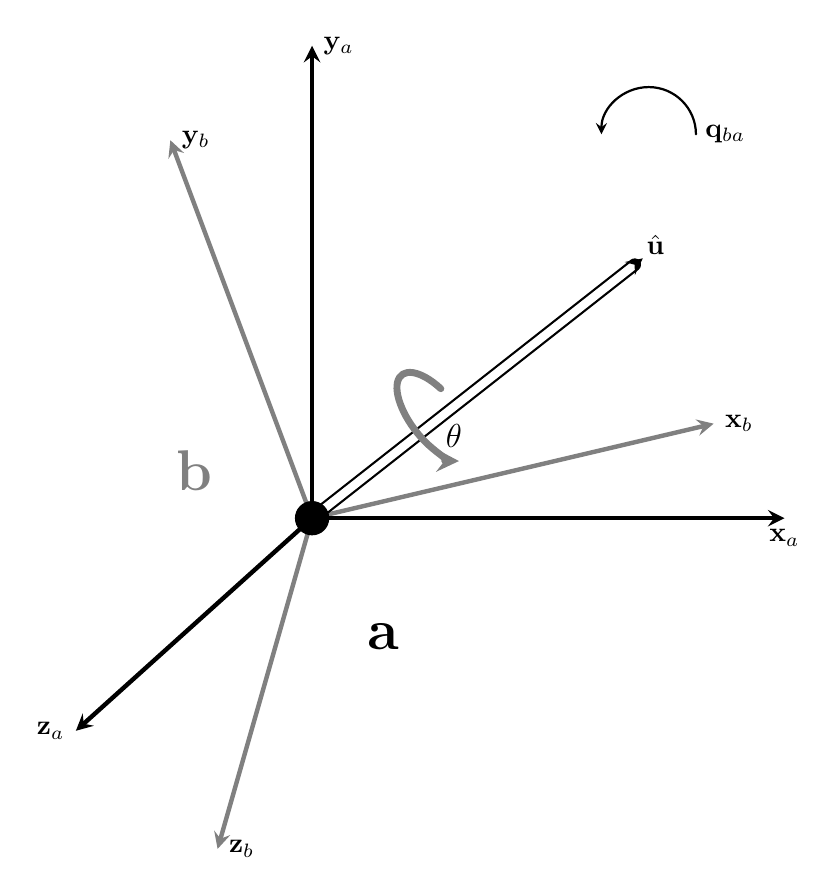
\begin{tikzpicture}[>=stealth, scale=1.5, line cap=round, line join=round]

    % ------------------------------------------------------------------
    % 1. Frame b (Rotated Frame)
    % Drawn first so it sits slightly behind the origin and Frame a
    % ------------------------------------------------------------------
    \draw[->, ultra thick, gray] (0,0) -- (3.4, 0.8) 
        node[right, text=black] {$\mathbf{x}_b$};
    \draw[->, ultra thick, gray] (0,0) -- (-1.2, 3.2) 
        node[right, text=black] {$\mathbf{y}_b$};
    \draw[->, ultra thick, gray] (0,0) -- (-0.8, -2.8) 
        node[right, text=black] {$\mathbf{z}_b$};

    % ------------------------------------------------------------------
    % 2. Frame a (Initial Frame)
    % ------------------------------------------------------------------
    \draw[->, ultra thick, black] (0,0) -- (4,0) 
        node[below] {$\mathbf{x}_a$};
    \draw[->, ultra thick, black] (0,0) -- (0,4) 
        node[right] {$\mathbf{y}_a$};
    \draw[->, ultra thick, black] (0,0) -- (-2,-1.8) 
        node[left] {$\mathbf{z}_a$};

    % ------------------------------------------------------------------
    % 3. Unit Rotation Axis (u)
    % Uses a double line to mimic the thick outline arrow in the image
    % ------------------------------------------------------------------
    \draw[->, double=white, double distance=3pt, thick, black] 
        (0,0) -- (2.8, 2.2) 
        node[above right, text=black, font=\bfseries, inner sep=1pt] {$\hat{\mathbf{u}}$};

    % ------------------------------------------------------------------
    % 4. Origin Marker (Drawn last to cover line intersections cleanly)
    % ------------------------------------------------------------------
    \filldraw[black] (0,0) circle (4pt);

    % ------------------------------------------------------------------
    % 5. Frame Identifiers (a and b)
    % ------------------------------------------------------------------
    \node[font=\huge\bfseries, black] at (0.6, -1.0) {a};
    \node[font=\huge\bfseries, gray] at (-1.0, 0.4) {b};

   % ------------------------------------------------------------------
    % 6. Theta rotation about the axis u (perpendicular perspective)
    % ------------------------------------------------------------------
    % Center of the arc positioned along u at (1.26, 0.99)
    \begin{scope}[shift={(1.26, 0.99)}, rotate=128]
        \draw[->, line width=2.5pt, gray]
            (160:-.2cm and 0.2cm) arc[start angle=-70, end angle=160, x radius=0.45cm, y radius=0.2cm];
    \end{scope}
    
    % Label offset slightly from the arc center
    \node[font=\large] at (1.2, .7) {$\theta$};

    % ------------------------------------------------------------------
    % 7. Quaternion rotation symbol (q_{b,a})
    % ------------------------------------------------------------------
    \draw[->, thick, black] 
        (3.25, 3.25) arc[start angle=0, end angle=180, radius=0.4] 
        node[pos=0, right, inner sep=3pt] {$\mathbf{q}_{ba}$};

\end{tikzpicture}
    \caption{Initial frame $a$, rotated frame $b$, unit rotation axis $\hat{\mathbf{u}}$, rotation angle $\theta$, and unit quaternion rotation $\mathbf{q}_{ba}$.}
    \label{fig:quaternion-rotation}
\end{figure}

A quaternion, \(\mathbf{q} \in \mathbb{H}\), consists of a scalar part \(q_s\) and a vector part \(\mathbf{q_v} = [q_x, q_y, q_z]^\mathsf{T} \in \mathbb{R}^3\) which together form a \ac{4-D} vector \cite{Diebel06,Schuster93} as depicted in \cref{fig:quaternion-rotation}.
Two conventions exist: a scalar first convention and a scalar last convention; this work utilizes the scalar last convention:
\begin{equation}
    \mathbf{q} = 
    \begin{bmatrix}
        q_x \\
        q_y \\
        q_z \\
        q_w
    \end{bmatrix}
    =
    \begin{bmatrix}
        \mathbf{q_v} \\
        q_s
    \end{bmatrix}
    = 
    \begin{bmatrix}
        sin(\theta/2) \hat{\mathbf{u}} \\
        cos(\theta/2)
    \end{bmatrix}
\label{eq:quaternion-scalar-last}
\end{equation}



Generally, quaternions both rotate \emph{and scale} vectors. 
However, a subset of quaternions, known as \emph{unit quaternions}, only rotate vectors without scaling them. 
Unit quaternions satisfy:
\begin{equation}
    \norm{\mathbf{q}}{2} = \sqrt{ q_x^2 + q_y^2 + q_z^2 + q_w^2} = 1.
\label{eq:unit-quaternion}
\end{equation}

The unit norm constraint is a critical property of our optimizations ensuring that the quaternions represent valid elements of \ac{SO3}.

Quaternion multiplication is used to represent relative rotations between orientations, where \(\mathbf{q}_{\text{relative}}\) transforms the initial frame into the identity orientation, represented by the identity quaternion $\mathbf{q}_{\text{identity}} = [\mathbf{0}_{3 \times 1}^\mathsf{T}, 1]^\mathsf{T}$.
\begin{equation}
    \overline{\mathbf{q}} = 
    \begin{bmatrix}
        -\mathbf{q_v} \\
        q_s
    \end{bmatrix},
\label{eq:quaternion-conjugate}
\end{equation}
\begin{equation}
    \mathbf{q}^{-1} = 
    \frac{\overline{\mathbf{q}}}{\norm{\mathbf{q}}{2}^2}.
\label{eq:quaternion-inverse}
\end{equation}
For unit quaternions the inverse equals the conjugate, i.e., $\mathbf{q}^{-1} = \overline{\mathbf{q}}$. The relative rotation quaternion is then:
\begin{equation}
    \mathbf{q}_{\text{relative}} = \mathbf{q}_{\text{initial}}^{-1} \otimes \mathbf{q}_{\text{final}},
\label{eq:relative-quaternion}
\end{equation}

\begin{equation}
\mathbf{q}_1 \otimes \mathbf{q}_2 =
\begin{bmatrix}
    q_{s,1} \mathbf{q}_{v,2} + q_{s,2} \mathbf{q}_{v,1} + \mathbf{q}_{v,1} \times \mathbf{q}_{v,2} \\
    q_{s,1} q_{s,2} - \mathbf{q}_{v,1} \cdot \mathbf{q}_{v,2}
\end{bmatrix}
\label{eq:quaternion-multiplication}
\end{equation}


A relative quaternion, $\mathbf{q}_{\text{relative}}$, represents the quaternion that rotates from the initial orientation to the final orientation and is useful for the mapping of \ac{MRPs} to \ac{SO3}.

Quaternions have a property known as the \emph{double-cover}:
\begin{equation}
\mathbf{R}(\mathbf{q}) = \mathbf{R}(-\mathbf{q}) 
\in \mathrm{SO(3)},
\label{eq:double-cover}
\end{equation}
meaning that both represent the same rotation.
To avoid ambiguity in representing rotations, it is common practice to enforce a convention, such as requiring the scalar part of the quaternion to be non-negative, i.e., \(q_s \geq 0\).
\begin{equation}
    \mathbf{q} \rightarrow 
    \begin{cases}
        \mathbf{q}, & q_s \geq 0 \\
        -\mathbf{q}, & q_s < 0
    \end{cases}
\label{eq:quaternion-negation}
\end{equation}
Enforcing this convention ensures a unique representation for each rotation and obviates an optimized slew taking the longer path due to quaternion sign ambiguity.
Along with the unit norm constraints and the scalar last convention, quaternion negation functions as the final condition of canonical quaternion representation for this work. 
Enforcing these conditions is known as quaternion canonization.

A final utility function is the conversion from quaternions to rotation matrices:
\begin{equation}
R_{\mathrm{bi}}(q) =
\begin{bmatrix}
    q_w^2 + q_x^2 - q_y^2 - q_z^2 & 2(q_xq_y + q_wq_z) & 2(q_xq_z - q_wq_y) \\
    2(q_xq_y - q_wq_z) & q_w^2 - q_x^2 + q_y^2 - q_z^2 & 2(q_yq_z + q_wq_x) \\
    2(q_xq_z + q_wq_y) & 2(q_yq_z - q_wq_x) & q_w^2 - q_x^2 - q_y^2 + q_z^2
\end{bmatrix}.
\label{eq:quat2rot}
\end{equation}

Like rotation matrices, quaternions have their own set of pros and cons:
\paragraph{Pros}
\begin{itemize}
    \item Singularity-free: Avoids the inherent singularities present in all smooth minimal attitude representations, allowing for continuous and well-defined attitude representation on the entirety of \ac{SO3}.
    \item Computationally Efficient: Contain only four elements--far fewer parameters than rotation matrices--and rely purely upon algebraic operations for frame transformations, avoiding transcendental trigonometric functions.
    \item Smooth Interpolation: Allow for smooth interpolation between rotations using \ac{SLERP}.
\end{itemize}

\paragraph{Cons}
\begin{itemize}
    \item Unit Norm Constraint: Only unit quaternions represent valid rotations, necessitating normalization after numerical operations to maintain the unit norm. The unit norm constraint also poses challenges in optimization frameworks as the feasible set exists on a \ac{3-D} manifold in \ac{4-D} space.
    \item Double Cover: $q$ and $-q$ map to the same physical rotation, introducing ambiguity that must be managed via consistent canonization, especially in optimization algorithms to avoid taking longer paths around the sphere.
    \item Redundant: They use four elements versus the three element minimal representation. 
    \item Geometrically Confusing: Being four-dimensional hyperspheres, quaternions are not easily conceptualized in comparison to other attitude representations.
\end{itemize}

\paragraph{\ac{MRPs}}
\label{par:mrps}

\ac{MRPs} represent the final attitude representation discussed in this work, offering a three-parameter minimal parameterization of rotations derived as stereographic projections of the unit quaternion hypersphere onto a \ac{3-D} hyperplane \cite{Schuster93}.

\ac{MRPs} were introduced in this work to implement the \ac{IPSO} algorithm--which due to characteristics of how \ac{PSO} algorithms explore search spaces, made quaternions, which require the unit norm constraint, impractical for this algorithm class.

This representation is defined in terms of the rotation axis $\hat{\mathbf{u}}$ and the rotation angle $\theta$ \cite{Schuster93} as shown in \cref{fig:quaternion-rotation}:
\begin{equation}
\mathbf{p}(\theta, \hat{\mathbf{u}}) 
= 
\tan\left(\frac{\theta}{4}\right) \hat{\mathbf{u}}
=
\frac{\mathbf{q}_v}{1+q_w},
\label{eq:MRP-defintion}
\end{equation}

As a minimal representation, \ac{MRPs} avoid redundancy inherent to quaternions and rotation matrices, but succumb unavoidably to either singularities or discontinuities.
From \cref{eq:MRP-defintion}, it is evident that \ac{MRPs} become singular when the rotation angle $\theta$ approaches $2\pi$, as $\tan\left(\frac{\theta}{4}\right)$ approaches infinity.
If the angle of rotation is bounded less than $2\pi$, \ac{MRPs} provide a continuous, singularity-free representation of rotations; however, spacecraft maneuvers are not constrained as such and singularities may appear \cite{Schuster93}.
One common approach to mitigate this issue is to switch to the shadow set of \ac{MRPs} when the norm of the current set exceeds unity--occurring for rotations greater than $\pi$--effectively avoiding the singularity at $2\pi$, but this introduces instead a discontinuity that optimizers struggle to handle.

Conversion between \ac{MRPs} and quaternions or rotation matrices occur via:
\begin{equation}
    \mathbf{q}(\mathbf{p}) = \frac{1}{1 + p^2} 
    \begin{bmatrix} 
        2\mathbf{p} \\
        1 - p^2 
    \end{bmatrix}
\label{eq:MRP2quat}
\end{equation}
\begin{equation}
    R_{bi}(\mathbf{p}) = 
    I_{3 \times 3} - \frac{4(1 - p^2)}{(1 + p^2)^2}[\mathbf{p}]_\times + \frac{8}{(1 + p^2)^2}[\mathbf{p}]_\times^2
\label{eq:MRP2rot}
\end{equation}

Naturally, \ac{MRPs} come with their own set of tradeoffs:

\paragraph{Pros}
\begin{itemize}
    \item Minimal Representation: Uses exactly three parameters to describe three \ac{DOF} rotations, eliminating the unit-norm constraint required by quaternions.
    \item Extended Singularity: As opposed to classic Rodrigues parameters, \ac{MRPs} exhibit singularities only at rotations of $2\pi$ rather than $\pi$, providing a larger singularity-free region for practical rotations.
    \item Transcendental-free Kinematics: Unlike Euler angles, the kinematic differential equations for \ac{MRPs} do not involve trigonometric functions.
\end{itemize}

\paragraph{Cons}
\begin{itemize}
    \item Singular or Discontinuous: Avoiding singularities involves switching to the shadow set for rotations greater than $\pi$, which can introduce discontinuities; without the shadow set, the representation is smooth but contains singularities.
    \item Spatial Warping: Due to \ac{MRPs} being a \emph{stereographic projection} of a \ac{4-D} hypersphere onto a \ac{3-D} hyperplane, straight paths in the MRP space  \emph{generally} do not correspond geodesics (great circles) on \ac{SO3}; a straight line trajectory only yields a true geodesic if the trajectory passes through the origin ($\mathbf{p}=\mathbf{0}$) and typically requires the use of relative rotations between coordinate frames to help align maneuvers with the origin. The distortion induces a change in the loss landscape, which affects optimization and control strategies.
\end{itemize}

\subsection{Dynamic Systems \& Constraints}
\label{sec:methodology-dynamics}
\begin{itemize}
	\item[$\square$] \textbf{System models:} Formulate the equations of motion for the spacecraft attitude dynamics on $\SO{3}$.
	\item[$\square$] Because the equations of motion for two unit vectors \(\hat{\mathbf{I}}\) and \(\hat{\mathbf{B}}\) represent the 7-DOF robotic manipulator.
	\item[$\square$] \textbf{State and control bounds:} Explicitly define the state, input, and kinodynamic constraint envelopes for both systems.
	\item[$\square$] Specify actuator limits, joint bounds, angular-velocity limits, and angular-acceleration limits for the spacecraft and manipulator as applicable.
\end{itemize}

\subsection{Optimal Control Problem (OCP) \& Nonlinear Programming Formulation}
\label{sec:methodology-ocp}
\begin{itemize}
	\item[$\square$] \textbf{OCP formulation:} Formalize the continuous-time optimal control problem, including the objective function, path constraints, and endpoint constraints.
	\item[$\square$] \textbf{NLP formulation:} Describe the transcription of the continuous-time OCP into a discrete nonlinear program (NLP).
	\item[$\square$] \textbf{Trajectory parameterization:} Detail the B-spline parameterization of the control and state trajectories.
	\item[$\square$] \textbf{Optimization framework:} Briefly describe IPOPT's role as the underlying interior-point NLP solver.
	\item[$\square$] Focus the IPOPT discussion on the interface, discretization of the continuous representation, and constraint handling rather than re-explaining IPOPT's internal algorithm.
\end{itemize}

\subsection{Algorithm Frameworks}
\label{sec:methodology-algorithms}
Present the four comparative trajectory-generation approaches with a consistent structure:
\begin{itemize}
	\item[$\square$] \textbf{MC-GBO:} Monte Carlo Gradient-Based Optimization.
	\item[$\square$] \textbf{RRT*-GBO:} Rapidly-exploring Random Tree Star combined with Gradient-Based Optimization.
	\item[$\square$] \textbf{P-HO:} Probabilistic Homotopy Optimization.
	\item[$\square$] \textbf{IPSO:} Inverse Dynamics Particle Swarm Optimization.
	\item[$\square$] For each approach, describe the initialization, sampling or warm-start mechanism, optimization phase, constraint treatment, and resulting trajectory representation.
	\item[$\square$] Include the $\SO{3}$ sampling mechanisms, distinguishing naive sampling from uniform sampling on $\SO{3}$.
	\item[$\square$] Include the sampling bounds used for the Arm7 manipulator.
\end{itemize}

\subsection{Adaptive Constraint Refinement}
\label{sec:methodology-refinement}
\begin{itemize}
	\item[$\square$] Detail the iterative refinement pipeline for B-spline trajectories.
	\item[$\square$] Describe how kinodynamic and boundary-constraint violations are detected along the continuous B-spline trajectories.
	\item[$\square$] Describe how time-grid nodes are locally densified around detected violations.
	\item[$\square$] Explain how local refinement enforces feasibility without global over-discretization.
\end{itemize}

\subsection{Analytical Verification}
\label{sec:methodology-verification}
\begin{itemize}
	\item[$\square$] \textbf{Analytical proof / baseline verification:} Present the unconstrained $\SO{3}$ maneuver proof.
	\item[$\square$] Use this proof as a mathematical validation that the baseline formulation and solver setup yield exact optimal solutions before evaluating complex constrained scenarios in Chapter~5.
\end{itemize}
